\documentclass[12pt]{exam}
\usepackage{amsthm}
\usepackage{bm}
\usepackage{libertine}
\usepackage[utf8]{inputenc}
\usepackage[margin=0.5in]{geometry}
\usepackage{amsmath,amssymb}
\usepackage{multicol}
\usepackage[shortlabels]{enumitem}
\usepackage{siunitx}
\usepackage{physics}
\usepackage{booktabs}
\usepackage{graphicx}
\usepackage{pgfplots}
\usepackage{listings}
\usepackage{tikz}
\usepackage{tikz-3dplot}
\usetikzlibrary{arrows.meta,decorations.markings}

\bmdefine{\ii}{i}
\bmdefine{\jj}{j}
\bmdefine{\kk}{k}
\newcommand{\te}{\theta}
\newcommand{\cC}{\mathcal{C}}
\newcommand{\word}[1]{\quad\text{#1}\quad}

\pgfplotsset{width=10cm,compat=1.9}
\usepgfplotslibrary{external}
\tikzexternalize
% Compile the small black-and-white solution diagram inline.
\tikzexternaldisable

\newcommand{\class}{Math 261-001}
\newcommand{\examnum}{Quiz 7 Solutions}
\newcommand{\examdate}{October 23}

\begin{document}
\pagestyle{plain}
\thispagestyle{empty}

\noindent
\textbf{\class}\\
\textbf{\examnum}, \textbf{\examdate}

\vspace{8pt}
\small
\setlength{\abovedisplayskip}{6pt}
\setlength{\belowdisplayskip}{6pt}
\setlength{\abovedisplayshortskip}{3pt}
\setlength{\belowdisplayshortskip}{6pt}
\begin{enumerate}

\item \textbf{Final answers:}
\[
  \boxed{(a,b)=(1,1)},\qquad
  \boxed{f(x,y,z)=x^2y+xz^2+yz+C}.
\]
The components of $\vec F_{a,b}$ are polynomials on all of
$\mathbb R^3$, so the field is conservative exactly when its curl is
identically zero. Compute
\[
\begin{aligned}
  \nabla\times\vec F_{a,b}
  &=\left(
     \frac{\partial}{\partial y}(2xz+y)
       -\frac{\partial}{\partial z}(bx^2+z),\
     \frac{\partial}{\partial z}(2xy+az^2)
       -\frac{\partial}{\partial x}(2xz+y),\
     \frac{\partial}{\partial x}(bx^2+z)
       -\frac{\partial}{\partial y}(2xy+az^2)
     \right)\\
  &=\bigl(0,\ 2(a-1)z,\ 2(b-1)x\bigr).
\end{aligned}
\]
For this to vanish at every point, we must have $a=b=1$.
For those values, integrate $f_x=2xy+z^2$ with respect to $x$:
\[
  f=x^2y+xz^2+g(y,z).
\]
The equation $f_y=x^2+z$ gives $g_y=z$, hence
$g(y,z)=yz+h(z)$. Finally, $f_z=2xz+y$ gives $h'(z)=0$.
Thus $h=C$, and direct differentiation verifies
\[
  \nabla(x^2y+xz^2+yz+C)
    =(2xy+z^2,\ x^2+z,\ 2xz+y)=\vec F_{1,1}.
\]

\medskip
\item \textbf{Final answers:}
\[
  \boxed{\displaystyle\oint_C\vec F\cdot\vec T\,ds=-6},\qquad
  \boxed{\displaystyle\oint_C\vec F\cdot\vec N\,ds=6}.
\]
Write $\vec F=(P,Q)$, where $P=y^3-2y$ and $Q=-4x+3y^2$.
The enclosed rectangle $D$ has bounds
\[
  \left\{
  \begin{aligned}
    &0\leq x\leq2,\\
    &0\leq y\leq1.
  \end{aligned}
  \right.
\]
Because $C$ is counterclockwise and $\vec T$ follows its orientation,
the circulation form of Green's theorem gives
\[
\begin{aligned}
  \oint_C\vec F\cdot\vec T\,ds
    &=\iint_D(Q_x-P_y)\,dA\\
    &=\int_0^2\int_0^1\bigl[-4-(3y^2-2)\bigr]\,dy\,dx\\
    &=\int_0^2[-2y-y^3]_0^1\,dx
     =\int_0^2(-3)\,dx=-6.
\end{aligned}
\]
For the outward unit normal $\vec N$, use the flux form instead:
\[
\begin{aligned}
  \oint_C\vec F\cdot\vec N\,ds
    &=\iint_D(P_x+Q_y)\,dA
      =\int_0^2\int_0^1 6y\,dy\,dx\\
    &=\int_0^2[3y^2]_0^1\,dx
     =\int_0^2 3\,dx=6.
\end{aligned}
\]
Circulation uses $Q_x-P_y$; outward flux uses the divergence $P_x+Q_y$.

\newpage

\item \textbf{Final answer:} $\boxed{4(xy+yz+xz)}$.

First compute the curl of $\vec G=(z^2,x^2,y^2)$:
\[
  \nabla\times\vec G
   =\bigl(2y-0,\ 2z-0,\ 2x-0\bigr)
   =(2y,2z,2x).
\]
Apply the divergence product rule with $\vec H=\nabla\times\vec G$:
\[
  \nabla\cdot(f\vec H)=\nabla f\cdot\vec H+f\,\nabla\cdot\vec H.
\]
Here $\nabla f=(2x,2y,2z)$, and
$\nabla\cdot(\nabla\times\vec G)=0$. Therefore
\[
\begin{aligned}
  \nabla\cdot\bigl(f(\nabla\times\vec G)\bigr)
    &=(2x,2y,2z)\cdot(2y,2z,2x)+f\cdot0\\
    &=4xy+4yz+4xz=4(xy+yz+xz).
\end{aligned}
\]
Although a curl has zero divergence, multiplying it by a nonconstant
scalar function introduces the term $\nabla f\cdot\vec H$.

\medskip
\item \textbf{Final answer:} $\boxed{5+\dfrac{\pi}{2}}$.

The given path $C$ is open. Add the downward segment $S$ from $(0,1)$
to $(0,0)$; then $C+S$ is the counterclockwise boundary of a region $D$.
For $P=ye^{xy}-y$ and $Q=xe^{xy}+x+1$,
\[
\begin{aligned}
  Q_x&=e^{xy}+xye^{xy}+1,\qquad
  P_y=e^{xy}+xye^{xy}-1,\\
  Q_x-P_y&=2.
\end{aligned}
\]

\noindent\begin{minipage}[c]{0.55\linewidth}
The region is a $2\times1$ rectangle together with a quarter disk of
radius $1$ centered at $(2,0)$. Thus
\[
  \operatorname{Area}(D)=2+\frac{\pi}{4}.
\]
Green's theorem gives
\[
  \int_C\vec F\cdot d\vec r+\int_S\vec F\cdot d\vec r
    =2\left(2+\frac{\pi}{4}\right)
    =4+\frac{\pi}{2}.
\]
\end{minipage}\hfill
\begin{minipage}[c]{0.41\linewidth}
\centering
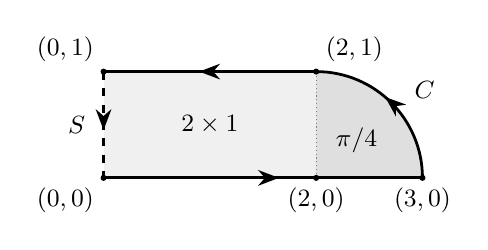
\begin{tikzpicture}[x=1.35cm,y=1.35cm,>=Stealth,
  directed/.style={line width=1pt,postaction={decorate},
    decoration={markings,mark=at position 0.55 with {\arrow{Stealth}}}},
  every node/.style={font=\small}]
  \fill[gray!12] (0,0) rectangle (2,1);
  \fill[gray!25] (2,0) -- (3,0)
    arc[start angle=0,end angle=90,radius=1] -- cycle;
  \draw[gray,densely dotted] (2,0) -- (2,1);
  \draw[directed] (0,0) -- (3,0);
  \draw[directed] (3,0) arc[start angle=0,end angle=90,radius=1];
  \draw[directed] (2,1) -- (0,1);
  \draw[dashed,directed] (0,1) -- (0,0);
  \node[left] at (-0.08,0.5) {$S$};
  \node at (1,0.5) {$2\times1$};
  \node at (2.38,0.35) {$\pi/4$};
  \node at (3.02,0.83) {$C$};
  \fill (0,0) circle (1.1pt) node[below left] {$(0,0)$};
  \fill (3,0) circle (1.1pt) node[below] {$(3,0)$};
  \fill (2,0) circle (1.1pt) node[below] {$(2,0)$};
  \fill (2,1) circle (1.1pt) node[above right] {$(2,1)$};
  \fill (0,1) circle (1.1pt) node[above left] {$(0,1)$};
\end{tikzpicture}
\end{minipage}

\medskip
On $S$, we have $x=0$, $dx=0$, and $y$ decreases from $1$ to $0$.
The second field component is $Q(0,y)=1$, so
\[
  \int_S\vec F\cdot d\vec r=\int_1^0 1\,dy=-1.
\]
Subtract this added segment's contribution to recover the original
open-path integral:
\[
  \int_C\vec F\cdot d\vec r
   =\left(4+\frac{\pi}{2}\right)-(-1)
   =5+\frac{\pi}{2}.
\]

\end{enumerate}
\end{document}
